%%%%%%%%%%%%%%%%%%%%%%%%%%%%%%%%%%%%%%%%%%%%%%%%%%%%%%%%%%%%%%%%%%%%%%%%%%%%%%%%
%%
%%   BornAgain User Manual
%%
%%   homepage:   http://www.bornagainproject.org
%%
%%   copyright:  Forschungszentrum Jülich GmbH 2015
%%
%%   license:    Creative Commons CC-BY-SA
%%
%%   authors:    Scientific Computing Group at MLZ Garching
%%               C. Durniak, M. Ganeva, G. Pospelov, W. Van Herck, J. Wuttke
%%
%%%%%%%%%%%%%%%%%%%%%%%%%%%%%%%%%%%%%%%%%%%%%%%%%%%%%%%%%%%%%%%%%%%%%%%%%%%%%%%%


\chapter{DWBA for multilayer systems}  \label{sec:Multilayers}


\index{Multilayer|(}%
\index{Layer structures|see {Multilayer}}

In \cref{Swave21},
we have discussed wave propagation and scattering in 2$+$1 dimensional systems
that are translationally invariant in the horizontal $xy$ plane,
and have a vertical refractive index profile $\nz(z)$.
Here we specialize to layered systems
where $\nz(z)$ is a step function that is constant within one layer.
First, only scalar interactions are considered.
Later, the theory is extended to account for polarization effects.

\Note{\indent By convention,
layers are numbered from top to bottom (see \cref{Fdefz}).
The top vacuum (or air) layer (which extends to $z\to+\infty$) has number~0,
\index{Multilayer!numbering}%
\index{Layer!index}%
the substrate (extending to $z\to-\infty$) is layer~$N$.}

All layer interfaces are assumed to be perfectly smooth.
% TODO RESTORE TEMPORARILY REMOVED XREF:
Support for rough interfaces is already implemented in \BornAgain,
but documentation is adjourned to a later edition of this manual.
% For rough interfaces, see \cref{sec:Roughness}.

%===============================================================================
\section{Wave propagation}\label{Slayerprop}
%===============================================================================

To compute scattering cross sections in DWBA,
we first need to determine the distorted wavefunctions~$\psi_w(\r)$
for $\r$ inside the sample.
The following derivation holds for the incoming wave ($w=\ti$)
as well as for the back-traced detected wave ($w=\tf$).

\begin{figure}[tb]
\begin{center}
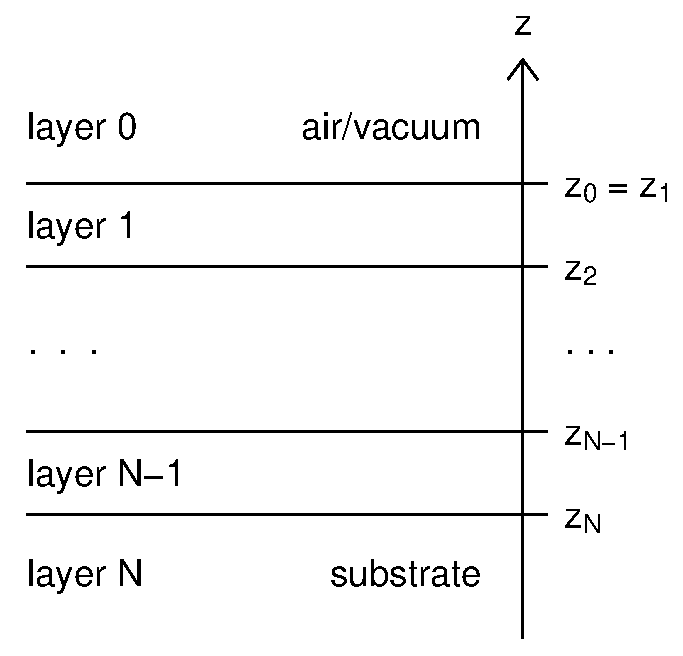
\includegraphics[width=0.4\textwidth]{fig/drawing/multilayer_z_conventions.ps}
\end{center}
\caption{The parameter $z_l$ is the $z$ coordinate of the \E{top} interface
\index{Multilayer!numbering}%
\index{Layer!index}%
\index{Multilayer!coordinates}%
\index{Layer!coordinate}%
of layer~$l$, except for $z_0$ which is the coordinate of the \E{bottom} interface
of the air or vacuum layer~0.}
\label{Fdefz}
\end{figure}

We consider wave propagation in one layer~$\il$
\nomenclature[2l020]{$\il$}{Index of layer in multilayer sample}%
with constant average refractive index $\nz(z)=\nzj$.
A vacuum plane wave, impinging on a layered structure,
is at each interface partly reflected, partly refracted,
so that the wavefunction inside a material layer
has an upward and a downward propagating component,
as per~\cref{Epsipm}.
Each component is a plane wave,
with a wavevector
\begin{equation}\label{Ekpmwj3}
  \k^\pm_{w\il}= \k_{\plll w} \pm k_{\perp w\il}\v{\hat z}.
\end{equation}
\nomenclature[2z060]{$\v{\hat z}$}{Unit vector along the sample normal}%
\nomenclature[2k043 2w010 2l010 \pm]{$\k^\pm_{w\il}$}{wavevector of the plane wave $\psi^\pm_{w\il}(\r)$}%
As explained in connection with~\cref{Ekpar},
the in-plane wavevector $\k_{\plll w}$ remains constant
across layer interfaces.
The vertical wavenumber is obtained from \cref{Ewavez},
\begin{equation}\label{Ekperpwj}
  k_{\perp w\il} = \sqrt{K^2 \nzj - k_{\plll w}^2}.
\end{equation}
In \cref{Smulayabs} we will discuss how to interpret this expression
in the case of a negative or complex radicand.
All of the following, unless explicitly restricted to real wavenumbers,
allows for complex values of~$k_\perp$.

We factorize the corresponding wavefunctions as
\begin{equation}\label{Eplawafa}
  \psi^\pm_{w\il}(\r)=\e^{i\k_{\plll w}\r_\plll}\phi^\pm_{w\il}(z),
\end{equation}
with vertical propagation described by a one-dimensional wavefunction
\begin{equation}\label{Ephizwj}
  \phi^\pm_{w\il}(z)=A^\pm_{w\il}\e^{\pm ik_{\perp w\il}(z-z_\il)}.
\end{equation}
\nomenclature[2a123 2w010 2l010 \pm]{$A^\pm_{w\il}$}{Amplitude of the plane wave $\phi^\pm_{w\il}(\r)$}%
For later convenience,
the phase factor in \cref{Ephizwj} includes an offset~$z_\il$
as defined in \cref{Fdefz}.
\nomenclature[2z020 2l010]{$z_l$}{Vertical coordinate at the top of layer~$l$ (at the bottom for $l=0$)}%
\index{Multilayer!coordinates}%
\index{Layer!coordinate}%
The amplitudes $A^\pm_{wl}$ need to be computed recursively,
as described below in \cref{Sacrolay}.

%===============================================================================
\section{Refraction, absorption, flux}\label{Smulayabs}
%===============================================================================

In the absence of absorption and above the critical angle,
wavevectors are real
so that we can describe the beam in terms of a glancing angle
\begin{equation}\label{Edef_alpha}
  \alpha_{w\il}\coloneqq \arctan(k_{\perp w\il}/k_{\plll w}).
\end{equation}
Equivalently,
\begin{equation}
  k_{\plll w}=K n_\il \cos\alpha_{w\il}.
\end{equation}
Since $k_{\plll w}$ is constant across layers,
we have
\begin{equation}\label{ESnell}
  n_\il \cos\alpha_{w\il} = \text{the same for all }\il,
\end{equation}
which is Snell's refraction law.
\index{Refraction!Snell's law}
\index{Snell's law}

In general, however, the vertical wavenumber $k_{\perp}$,
given by \cref{Ekperpwj},
can become imaginary or complex.
This makes the above geometric interpretation untenable.
Yet the algebraic formalism developed in \cref{Slayerprop}
remains applicable.
The horizontal wavevector $\k_\plll$ remains constant and real
as initialized somewhere above the sample.
However, the radicand in \cref{Ekperpwj} can become
negative (total reflection conditions) or complex
(absorbing layer,
with a positive imaginary part of $\overline{n^2}$).
In both cases, the vertical wavevector component $k_{\perp}$
becomes complex.
\index{Wavevector!complex}%
We write
\begin{equation}\label{decompkperp}
  k_\perp \eqqcolon k_\perp' + i k_\perp''
\end{equation}
for its decomposition into a real and an imaginary part.
With \cref{Endb1}, $\beta\ge0$ and $\delta<1$,
we always have $k_\perp'\cdot k_\perp''\ge0$.
In analogy with \cref{decompkperp},
full wavevectors have the decomposition
\begin{equation}
  \k^\pm
  \eqqcolon {\k^\pm}' + i{\k^\pm}''
  = \k_\plll \pm (k_\perp' + i k_\perp'')\v{\hat z}.
\end{equation}
After these preparations,
we can compute the flux~\cref{EdefJ}
associated with the plane-wave solution (\ref{Eplawafa},\ref{Ephizwj}):
\begin{equation}
  \begin{array}{@{}l@{\;}l}
  \v{J}(\r)
  =&   \left|A^-\right|^2 \e^{+2k_\perp'' (z-z_l)} {\k^-}'
    + \left|A^+\right|^2 \e^{-2k_\perp''(z-z_l)} {\k^+}'
\\[2ex]
  &+ \left[
      A^-{A^+}^* \e^{-2ik_\perp'(z-z_l)} {\left(\k_\plll-ik_\perp''\v{\hat z}\right)}
    + \text{c.c.}
    \right].
  \end{array}
\end{equation}
The first two terms describe the exponential intensity decrease
due to absorption, while
the oscillatory term in square brackets
is responsible for waveguide effects in layers with finite thickness.

The flux can also be written in terms of the one-dimensional wavefunctions $\phi^{\pm}(z)$:
\begin{equation}
  \begin{array}{@{}l@{\;}l}
  \v{J}(\r) =& \left|\phi^+(z)+\phi^-(z)\right|^2\cdot\k_\plll \\
  &+ \left[ \left|\phi^+(z)\right|^2 k_\perp' - \left|\phi^-(z)\right|^2 k_\perp' +
  2\Im(\phi^-(z){\phi^+}^*(z))k_\perp'' \right]\cdot \v{\hat z}.
  \end{array}
\end{equation}
The first term denotes the horizontal component of the flux and can be seen to consist of the product
of the particle density at position $z$ and the wavector $\k_\plll$. The $z$-component consists of the difference between the up- and downward travelling wave components and an extra term that encodes the interference between them.

In the special case of a purely imaginary~$k_{\perp \il}$,
the flux becomes:
\begin{equation}
  \v{J}(\r) = \left| \psi \right|^2 \k_\plll + 2 \Im (A^-{A^+}^*) k_\perp''\v{\hat z}.
\end{equation}
This flux consists of two clearly distinct parts: an \E{evanescent wave},
\index{Evanescent wave}%
travelling horizontally
 and a vertical component that is independent of the $z$ position. The vertical component is a necessary
 degree of freedom to fulfill the boundary conditions at the layer's top and bottom interfaces.
In the case of a semi-infinite layer, the vertical component becomes zero and
 all incoming radiation at the top of the layer undergoes \E{total reflection}.
\index{Total reflection}%
%===============================================================================
\section{DWBA matrix element}
%===============================================================================

Since the $\psi^\pm_{w\il}$ are plane waves within layer~$\il$,
we can at once write down the DWBA transition matrix element~\cref{Edwba}
\index{Distorted-wave Born approximation!multilayer}%
\begin{equation}\label{Edwba_ml0}
  \bra \psi_\ti|\chi|\psi_\tf\ket
  = \sum_{\il} \sum_{\pm_\ti} \sum_{\pm_\tf}
    A^{\pm *}_{\ti \il} A^\pm_{\tf \il}
     \chi_\il(\k^\pm_{\tf \il}-\k^\pm_{\ti \il}),
\end{equation}
where
\begin{equation}\label{Echij}
  \chi_\il(\v{q})
  \coloneqq  \int_{z_\il}^{z_{\il-1}}\!\d z \int\!\d^2r_\plll\, \e^{i\v{q}\,\r}\chi(\r)
\end{equation}
\nomenclature[1χ032 2l010 2q040]{$\chi_\il(\v{q})$}{Fourier transform of the perturbation potential $\chi(\r)$, evaluated in one sample layer}%
is the Fourier transform
of the perturbative potential~\cref{EChiGraded},
restricted to one layer.

To alleviate later calculations,
we now number the four DWBA terms from 1 to~4,
and define the corresponding wavenumbers and amplitude factors and as
\begin{equation}
  \begin{array}{l@{\hspace{2em}}l}
    \q^1 \coloneqq  \k^-_\tf - \k^-_\ti,& C^1 \coloneqq  A^{-*}_\ti A^-_\tf, \\[.6ex]
    \q^2 \coloneqq  \k^-_\tf - \k^+_\ti,& C^2 \coloneqq  A^{-*}_\ti A^+_\tf, \\[.6ex]
    \q^3 \coloneqq  \k^+_\tf - \k^-_\ti,& C^3 \coloneqq  A^{+*}_\ti A^-_\tf, \\[.6ex]
    \q^4 \coloneqq  \k^+_\tf - \k^+_\ti,& C^4 \coloneqq  A^{+*}_\ti A^+_\tf.
  \end{array}
\end{equation}
Accordingly, we can write \cref{Edwba_ml0} as
\Emph{
\begin{equation}\label{Edwba_ml}
  \bra \psi_\ti|\chi|\psi_\tf\ket
  = \sum_{\il} \sum_{u} C^u_\il \chi_\il(\q_\il^u).
\end{equation}
\vspace*{-5pt}}
From~\cref{Ekpmwj3} we see that all four wavevectors $\q^u$
have the same horizontal component,
\begin{equation}\label{Eqpp}
  \q^u = \q_\plll + q^u_\perp \v{\hat z}
\end{equation}
whence the vertical components
\begin{equation}
    \begin{array}{l}
  q^1_\perp = +k_{\tf\perp  } -k_{\ti\perp},\\[.6ex]
  q^2_\perp = +k_{\tf\perp  } +k_{\ti\perp},\\[.6ex]
  q^3_\perp = -k_{\tf\perp  } -k_{\ti\perp},\\[.6ex]
  q^4_\perp = -k_{\tf\perp  } +k_{\ti\perp}.
    \end{array}
\end{equation}

%===============================================================================
\section{Wave propagation across layers}\label{Sacrolay}
%===============================================================================

\index{Fresnel coefficients}%
\index{Transmission|see {Fresnel coefficients}}%
\index{Reflection|seealso {Fresnel coefficients}}%

The plane-wave amplitudes $A^\pm_{w\il}$ need to be computed recursively
from layer to layer.
Since these computations are identical for incident and final waves,
we omit the subscript~$w$ in the remainder of this section.
At layer interfaces, the optical potential changes discontinuously.
From elementary quantum mechanics we know that
piecewise solutions of the Schrödinger equations must be connected
such that the wavefunction $\phi(\r)$ and its first derivative
$\Nabla\phi(\r)$ evolve continuously.

\begin{figure}[tb]
\begin{center}
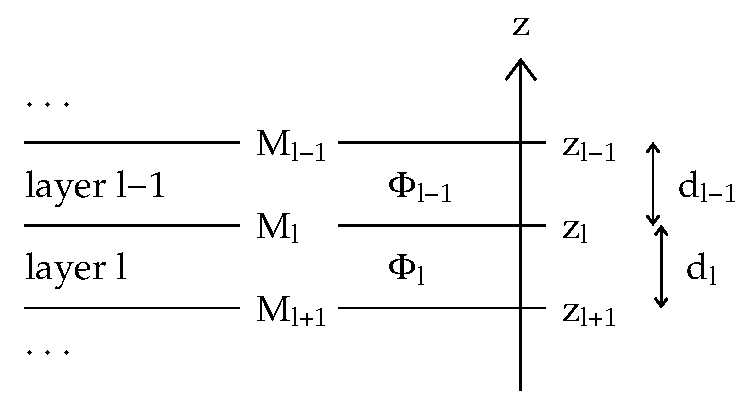
\includegraphics[width=0.46\textwidth]{fig/drawing/multilayer_boundary.ps}
\end{center}
\caption{The transfer matrix $M_l$ connects the wavefunctions
\index{Multilayer!transfer matrix}%
\index{Layer!transfer matrix}%
\index{Transfer matrix}%
$\Phi_l$, $\Phi_{l-1}$ in adjacent layers.}
\label{Fboundary}
\end{figure}

To deal with the coordinate offsets introduced in \cref{Ephizwj},
we introduce the function%
\begin{equation}
  d_\il\coloneqq z_{\il}-z_{\il+1},
\end{equation}
which is the thickness of layer~$\il$,
except for $\il=0$,
where the special definition of $z_0$ (\cref{Fdefz}) implies $d_0=0$.
We consider the interface between layers $\il$ and $\il-1$,
with~$\il=1,\ldots,N$, as shown in \cref{Fboundary}.
This interface has the vertical coordinate $z_{\il}=z_{l-1}-d_{l-1}$.
Accordingly, the continuity conditions at the interface are
\begin{equation}\label{Econtcond}
  \begin{array}{lcl}
 \hphantom{\partial_z}\phi_{\il}(z_{\il}) &=& \hphantom{\partial_z}\phi_{\il-1}(z_{\il-1}-d_{\il-1}),\\
           \partial_z \phi_{\il}(z_{\il}) &=&           \partial_z \phi_{\il-1}(z_{\il-1}-d_{\il-1}).
  \end{array}
\end{equation}
We abbreviate
\begin{equation}
  f_\il \coloneqq  k_{\perp \il}/K = \sqrt{\nzj-(k_\plll/K)^2}
\end{equation}
and
\begin{equation}
   \delta_\il \coloneqq  \e^{iKf_\il d_\il}.
\end{equation}
For the plane waves \cref{Ephizwj},
the continuity conditions~\cref{Econtcond} take the form
\begin{equation}\label{Econt2}
  \begin{array}{@{}l@{}lcl@{}l}
  +A^-_{\il} &+A^+_{\il}
  &=&
  +A^-_{\il-1}\delta_{\il-1} &+A^+_{\il-1}\delta_{\il-1}^{-1},
  \\
  -A^-_{\il} f_{\il}  &+A^+_{\il} f_{\il}
  &=&
  -A^-_{\il-1}\delta_{\il-1} f_{\il-1} &+A^+_{\il-1}\delta_{\il-1}^{-1} f_{\il-1}.
  \end{array}
\end{equation}
After some lines of linear algebra,
we can rewrite this equation system as
\begin{equation}\label{EcMc}
  \left( \begin{array}{c}A^-_{\il-1}\\ A^+_{\il-1}\end{array} \right)
  = M_{\il} \left( \begin{array}{c}A^-_{\il}\\A^+_{\il}\end{array} \right)
\end{equation}
with the transfer matrix
\begin{equation}\label{EMil}
  M_\il
   \coloneqq
   \left(\begin{array}{cc}
     \delta_{\il-1}^{-1}&0\\
       0 & \delta_{\il-1}
   \end{array}\right)
   \frac{1}{2f_{\il-1}}
   \left(\begin{array}{cc}
       (f_{\il-1}+f_{\il})&(f_{\il-1}-f_{\il})\\
       (f_{\il-1}-f_{\il})&(f_{\il-1}+f_{\il})
   \end{array}\right).
\end{equation}

In a scattering setup,
plane-wave amplitudes are subject to two boundary conditions.
Let us assume that the source or the sink is located at $z>0$.
Then in the top layer, $A^-_{0}=1$ is given by the
incident or back-traced final plane wave.
In the substrate, $A^+_{N}=0$ because there is no radiation
coming from $z\to-\infty$.
This leaves us with two unkown amplitudes,
the overall coefficients of transmission~$A^-_N$ and reflection~$A^+_0$.
These two unknowns are  connected by a system of two linear equations,
\begin{equation}
  \left( \begin{array}{c}1\\ A^+_0\end{array} \right)
  = M_1 \cdots M_{N} \left( \begin{array}{c}A^-_N\\0\end{array} \right).
\end{equation}
While it is possible in principle
to solve this as a matrix equation,
the actual implementation in \BornAgain\
%\footnote{SpectralMatrix.cpp: SpectralMatrix::execute()}
starts with a unit vector in the substrate,
and then carries out the propagation step \cref{EcMc}
interface by interface,
yielding unnormalized amplitudes
\begin{equation}\label{EAtildel}
  \left( \begin{array}{c}\tilde A^-_{\il}\\ \tilde A^+_{\il}\end{array} \right)
  \coloneqq M_{\il+1}\cdots M_{N} \left( \begin{array}{c}1\\0\end{array} \right).
\end{equation}
When the top layer is reached,
the obtained values are normalized
so that the boundary condition $A^-_{0}=1$ be satisfied,
\begin{equation}
  A^\pm_{\il} = \frac{\tilde A^\pm_l}{\tilde A^-_0}.
\end{equation}
For GISAS detection in transmission geometry
\index{Transmission geometry}%
\index{Detector!transmission geometry}%
(sink location $z<0$) all the development
following \cref{EMil} holds with exchanged order of layers:
$(0,\ldots, N) \mapsto (N,\ldots,0)$.

\Work{GISAS in transmission geometry is not yet implemented in \BornAgain,
  but high on our agenda.}

At this point,
it may be an interesting exercise to make
 a connection with a well known textbook result.
Consider a system
with a single interface between two semi-infinite,
non-absorbing media. The incoming wave is assumed to be above the
critical angle, ensuring all $f_l$ are real.
The reflected flux,
normalized to the incident vertical flux $J_{0\perp}^-=-Kf_0$,
is
\index{Reflected flux}%
\begin{equation}
  \frac{J_{0\perp}^+}{J_{0\perp}^-}
  = - \left(\frac{f_0-f_1}{f_0+f_1}\right)^2,
\end{equation}
and the transmitted flux
\index{Trasmitted flux}%
\begin{equation}
  \frac{J_{1\perp}^-}{J_{0\perp}^-}
  = \frac{4f_0 f_1}{(f_0+f_1)^2}.
\end{equation}
This satisfies particle number conservation, $J_{0\perp}^-+J_{0\perp}^+=J_{1\perp}^-$,
and agrees with Fresnel's result for $s$-polarized light.\footnote
{See any optics textbook, e.g.\ Born~\&~Wolf \cite[ch.~1.5.2]{BoWo99}
  or Hecht \cite[ch.~4.6.2]{Hec02}.}

The above algorithm fails if $f_{\il}\to0$
because $M_{\il+1}$ becomes singular.
The general solution of \cref{Ewavez} will be a linear function of $z$:
\begin{equation}
  \phi_{\il}(z) = A^0_{\il} + A^1_{\il}z.
\end{equation}
In \BornAgain, such a linear wavefunction amplitude can not be handled by the form factors,
which are only defined in terms of plane waves with complex wavevector components.
The following cases are treated seperately:
\begin{itemize}
  \item There is only one layer: this is a trivial case whithout any need to calculate wave coefficients.
    The solution in the single layer is just the incoming/outgoing plane wave.
  \item The top layer of a multilayer has $f_0=0$: the limit $f_0\to0$ is well-defined and the
    solution is given by $A^+_0 = -A^-_0$ and $A^{\pm}_{\il}=0$ for $\il>0$.
    % The boundary condition in the substrate imposes a linear relation between the two coefficients
    % of the linear wavefunction amplitude in the top layer. Since the first order term has to vanish, all amplitudes vanish.
  \item $f_{\il}=0$ for a layer with $\il>0$: In this case $f_{\il}$ will be given a very small imaginary value,
    representing a slight absorption. However, this should be inconsequential because the index of refraction
    of non-vacuum layer always contains an absorptive component.
\end{itemize}

\index{Multilayer|)}%
